\documentclass[11pt]{article}
\usepackage[margin=0.8in]{geometry}
\usepackage[]{amsfonts, amssymb, amsmath, float, hyperref,fancyheadings, graphicx, derivative}
\pagestyle{fancy}
\lhead{Data Analytic Tools}
\chead{Larry128}
\rhead{MATH3332}
\renewcommand{\footrulewidth}{0.4pt}
\setcounter{tocdepth}{3} % set TOC
\newcommand{\indep}{\perp \!\!\! \perp}

% codeblocks
\usepackage{listings}
\usepackage{xcolor}
\definecolor{codegreen}{rgb}{0,0.6,0}
\definecolor{codegray}{rgb}{0.5,0.5,0.5}
\definecolor{codepurple}{rgb}{0.58,0,0.82}
\definecolor{backcolour}{rgb}{0.95,0.95,0.92}
\lstdefinestyle{mystyle}{
    backgroundcolor=\color{backcolour},   
    commentstyle=\color{codegreen},
    keywordstyle=\color{magenta},
    numberstyle=\tiny\color{codegray},
    stringstyle=\color{codepurple},
    basicstyle=\ttfamily\footnotesize,
    breakatwhitespace=false,         
    breaklines=true,                 
    captionpos=b,                    
    keepspaces=true,                 
    numbers=left,                    
    numbersep=5pt,                  
    showspaces=false,                
    showstringspaces=false,
    showtabs=false,                  
    tabsize=3
}
\lstset{style=mystyle}
\lstdefinestyle{customc}{
  language=C++,
  % Add other settings here
}

%common math symbols
\newcommand{\R}{\mathbb{R}}
\newcommand{\N}{\mathbb{N}}
\newcommand{\Q}{\mathbb{Q}}
\newcommand{\C}{\mathbb{C}}
\newcommand{\ddx}{\dfrac{d}{dx}}
\newcommand{\regressf}{$f(\mathbf{x}; \mathbf{w})$ }
\newcommand{\lossf}{$L(\mathbf{w}; S)$ }
\newcommand{\vx}{\mathbf{x}}
\newcommand{\vy}{\mathbf{y}}
\newcommand{\vz}{\mathbf{z}}
\newcommand{\vzero}{\mathbf{0}}
\newcommand{\st}{\text{ s.t. }}

% asymptotic notations
\newcommand\BigO[1]{$O($#1$)$}
\newcommand\BigOmega[1]{$\Omega($#1$)$}
\newcommand\BigTheta[1]{$\Theta($#1$)$}
\newcommand\pddx[2]{\frac{\partial{#1}}{\partial{#2}}}

% pgfplots
\usepackage{pgfplots}
\pgfplotsset{compat=1.18, width=8cm}
\usepackage{geometry}
\geometry{
a4paper,
total={170mm,257mm},
left=20mm,
top=20mm,
}
\usetikzlibrary{shapes.geometric}

\begin{document}
\begin{titlepage}
    \begin{center}
        \vspace*{1cm}
            
        \Huge
        \textbf{MATH3332}
            
        \vspace{0.5cm}
        \LARGE
        Data Analytic Tools
            
        \vspace{1.5cm}
            
        Larry128
            
        \vfill
            
        A summary notes for revision
            
        \vspace{0.8cm}
                
        \Large
        Fall 2024-2025
            
    \end{center}
\end{titlepage}
\tableofcontents
\newpage

\section{Vector Space, metric, limits/ convergence}
\subsection{Vector Spaces}
A vector space (linear space) over $\mathbb{R}$ (in real domain) is a set $V$ together with functions:
\begin{enumerate}
\item Vector addition \begin{align*}
(V, V) \mapsto V\\
\equiv (\mathbf{x}, \mathbf{y}) \in (V, V) \implies \mathbf{x} + \mathbf{y}
\end{align*}
\item Scalar multiplication \begin{align*}
(\mathbb{R}, V) \mapsto V\\
\equiv \forall \alpha \in \mathbb{R}, \mathbf{x} \in V, \alpha \mathbf{x} \in V
\end{align*}
\end{enumerate}
These two functions should satisfy the following $8$ properties. $\forall \vx, \vy, \vz \in V$
\begin{enumerate}
\item Associativity of addition \begin{align*}
\vx + \vy + \vz = \vx + (\vy + \vz) = (\vx + \vy) + \vz
\end{align*}
\item Commutativity of addition \begin{align*}
\vx + \vy = \vy + \vx
\end{align*}
\item Zero vector \begin{align*}
\exists \vzero \text{ s.t. } \vx + \vzero = \vzero + \vx
\end{align*}
\item Negative vector \begin{align*}
\forall \vx \in V, \exists -\vx \in V, \st \vx + (-\vx) = (-\vx) + \vx = \vzero
\end{align*}
\item \begin{align*}
 1 \dot \vx = \vx
\end{align*}
\item \begin{align*}
\forall \alpha, \beta \in \R, \alpha (\beta \vx) = (\beta \alpha) \vx
\end{align*}
\item \begin{align*}
\forall \alpha, \beta \in \R, (\alpha + \beta) \vx = \alpha \vx + \beta \vx
\end{align*}
\item \begin{align*}
\forall \alpha \in \R, \alpha (\vx + \vy) = \alpha \vx + \alpha \vy
\end{align*}
\end{enumerate}
Remarks: \begin{enumerate}
\item We can define vector space over the complex domain $\C$ similarly.
\item We will assume vector space in the real domain by default. Vector space over complex domain is used very rarely.
\end{enumerate}
\textbf{Examples of vector spaces}
\begin{enumerate}
\item $\R$ with standard addition of real numbers and the standard multiplication of real numbers is a vector space.
\item $\R^n$ $n$-dimensional Euclidean space with addition and multiplication defined as follows\\
Addition:
\begin{align*}
\vx = \begin{bmatrix}
x_1\\ x_2\\ \vdots\\ x_n
\end{bmatrix}, \vy = \begin{bmatrix}
y_1\\ y_2\\ \vdots\\ y_n
\end{bmatrix}, \vx + \vy = \begin{bmatrix}
x_1 + y_1\\ x_1 + y_2\\ \vdots\\x_n + y_n
\end{bmatrix}
\end{align*}
Multiplication:
\begin{align*}
\alpha \in \R, \vx = \begin{bmatrix}
x_1\\ x_2\\ \vdots\\ x_n
\end{bmatrix}, \alpha \vx = \begin{bmatrix}
\alpha x_1\\ \alpha x_2\\ \vdots\\ \alpha x_n
\end{bmatrix}
\end{align*}
Zero: $$ \vzero = \begin{bmatrix}
0& 0& \dots& 0
\end{bmatrix}^T$$
Then, $\R^n$ is a vector space since it is closed in addition and scalar multiplication, and $\vzero \in \R^n$.
\item All real $m \times n$ matrices $\R^{m \times n}$ with addition and multiplication defined as:\\
Addition:
\begin{align*}
X = \begin{bmatrix}
x_{11} & x_{12}& \dots& x_{1n}\\
x_{21} & x_{22}& \dots& x_{2n}\\
\vdots & \vdots& \\
x_{m1} & x_{m2}& \dots& x_{mn}\\
\end{bmatrix}, 
Y = \begin{bmatrix}
y_{11} & y_{12}& \dots& y_{1n}\\
y_{21} & y_{22}& \dots& y_{2n}\\
\vdots & \vdots& \\
y_{m1} & y_{m2}& \dots& y_{mn}\\
\end{bmatrix}, X+Y = (x_{ij} + y_{ij})_{m \times n}
\end{align*}
Multiplication:
\begin{align*}
\alpha \in \R, X = \begin{bmatrix}
x_{11} & x_{12}& \dots& x_{1n}\\
x_{21} & x_{22}& \dots& x_{2n}\\
\vdots & \vdots& \\
x_{m1} & x_{m2}& \dots& x_{mn}\\
\end{bmatrix},  \alpha X = (\alpha x_{ij})_{m \times n}
\end{align*}
Zero: $$ \vzero = \begin{bmatrix}
0& 0& \dots& 0\\ 
0& 0& \dots& 0\\ 
\vdots& \vdots& \\
0& 0& \dots& 0\\ 
\end{bmatrix}$$
Then $\R^{m \times n}$ is a vector space.
Remarks: \begin{enumerate}
\item This vector space is same as $\R^{mn}$ by vectorization.
\item Vectorization $\R^{m \times n} \mapsto \R^{mn}$ \begin{align*}
\begin{bmatrix}
x_{11} & x_{12}& \dots& x_{1n}\\
x_{21} & x_{22}& \dots& x_{2n}\\
\vdots & \vdots& \\
x_{m1} & x_{m2}& \dots& x_{mn}\\
\end{bmatrix} \rightarrow \begin{bmatrix}
x_{11}\\
\vdots\\
x_{m1}\\
x_{12}\\
\vdots\\
x_{m2}\\
\vdots\\
x_{1n}\\
\vdots\\
x_{mn}\\
\end{bmatrix}
\end{align*}
\end{enumerate}
\item All real 3-array of size $m \times n \times n \times l$ $\R^{m \times n \times l}$ with addition and multiplication defined as\\
Addition: $$X = (x_{ijk})_{i, j, k}, Y = (y_{ijk})_{i, j, k} \in \R^{m \times n \times l}, X+Y = (x_{ijk} + y_{ijk})_{i, j, k} \in \R^{m \times n \times l}$$
Multiplication: $$\alpha \in \mathbb{R}, X = (x_{ijk})_{i, j, k} \in \R^{m \times n \times l}, \alpha X = (\alpha x_{ijk})_{i, j, k}$$
\item (Function space). The set of all continuous functions on [a, b], denoted by $$C[a, b] := \{ f : f \text{ is a continous function on } [a, b]\}$$ with addition defined as \begin{align*}
\forall f, g \in C[a, b], (f+g)(t) = f(t) + g(t) , \forall t \in [a, b]
\end{align*} and multiplication defined as \begin{align*}
\forall \alpha \in \R, f \in C[a, b], (\alpha f)(t) = \alpha f(t) \forall t \in [a, b]
\end{align*} is a vector space.
\end{enumerate}
\textbf{Counter-example of vector spaces}
\begin{enumerate}
\item Define $V = [-1, 1] \subset \R$. We can easily say that $V$ is not a vector space by considering a counter-example: $1+1 = 2 \notin V$.
\item Consider the set of all strings with addition defined as \texttt{'I' + ' am' = 'I am'}.  But this addition definition violates the commutativity of addition \texttt{"I" + " am" $\neq$ " am" + "I"}. \\ Therefore, we cannot use vector space to model text data in this naive way.
\end{enumerate}

\subsection{Metric on vector space}
Metric on vector space is to define the "closeness/ distance" of two vectors in order to do calculus on vector spaces.\\
Let $V$ be a vector space and $\vx, \vx \in V$, then $$\text{dist}(\vx, \vy) = \text{dist}(\vx -\vy) = \text{length of }\vx - \vy$$ and (triangular inequality) $$\text{dist} (\vx, \vy) + \text{dist}(\vy, \vz) \geq \text{dist} (\vx, \vz)$$
Remark: distance should be \textit{shift invariance}.\\
Therefore, to define distance, we only need to define the length (norm) of vectors.\\ Let $\vx \in V$. Denote $||\vx||$ be the length (norm) of $\vx$. Then $||\vx||$ should satisfy:
\begin{enumerate}
\item Non-negativity $$||\vx|| \geq 0$$ and $$||\vx|| = 0 \iff \vx = \vzero$$
\item Length of a scaling of a vector is a scaling of the length of the vector $$||\alpha \vx|| = |\alpha| ||\vx||$$ \begin{center}
\begin{tikzpicture}
\draw [-latex, black, thick] (0, 0) -- (1, 1) node[right]{$\vx$};
\draw [-latex, blue] (0, 0) -- (2, 2) node[right]{$\alpha \vx$ with $\alpha > 0$};
\draw [-latex, red] (0, 0) -- (-0.8, -0.8) node[left]{$\alpha \vx$ with $\alpha < 0$};
\end{tikzpicture}
\end{center}
\item (Triangular Inequality) $$||\vx + \vy|| \leq ||\vx|| + ||\vy||$$
\begin{center}
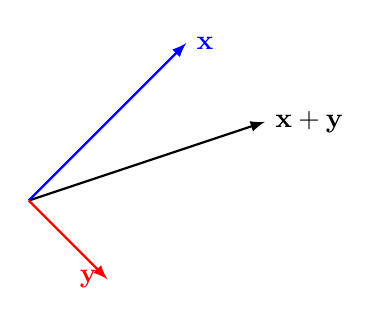
\begin{tikzpicture}
\draw [-latex, black, thick] (0, 0) -- (3, 1) node[right]{$\vx + \vy$};
\draw [-latex, blue, thick] (0, 0) -- (2, 2) node[right]{$\vx$};
\draw [-latex, red, thick] (0, 0) -- (1, -1) node[left]{$\vy$};
\end{tikzpicture}
\end{center}
\end{enumerate}
\textbf{Examples of vector norms}
\begin{enumerate}
\item Euclidean norm ($2-$ norm) $$||\vx||_2 = (\sum_{i=1}^{n} x_i^2)^{\frac{1}{2}}$$
\begin{enumerate}
\item $$\forall i \in \{1, 2, \cdots, n\},  x_{i}^2 \geq 0 \implies \sum_{i=1}^{n} x_i^2 \geq 0 \implies ||\vx||_2 \geq 0$$ and $$||\vx||_2 = 0 \iff (\sum_{i=1}^{n} x_i^2)^{\frac{1}{2}} = 0 \iff \sum_{i=1}^{n} x_i^2 = 0 \iff x_i =0, \forall i \in {1, 2, \cdots, n} \iff \vx = \vzero$$
\item $$||\alpha \vx||_2 = (\sum_{i=1}^{n} (\alpha x_i)^2)^{\frac{1}{2}} = (\sum_{i=1}^{n} \alpha^2 x_i^2)^{\frac{1}{2}} = (\alpha^2 \sum_{i=1}^{n} x_i^2)^{\frac{1}{2}} = |\alpha|(\sum_{i=1}^{n} x_i^2)^{\frac{1}{2}} = |\alpha|||\vx||_2$$
\item $$||\vx + \vy||_2 \leq ||\vx||_2 + ||\vy||_2$$ (To be proved later)
\end{enumerate}
\item $\infty -$norm $$||\vx||_{\infty} = \max_{i \in \{1, 2, \cdots, n\}} |x_i|$$
\item $p-$norm $$||\vx||_p = (\sum_{i=1}^{n} |x_i|^p)^{\frac{1}{p}}$$
Comparison of $p-$norms across different $p$
\begin{center}
\begin{tabular}{cc}
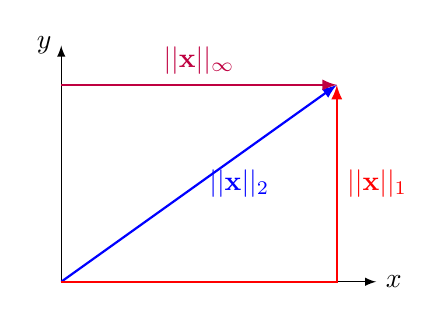
\begin{tikzpicture}
\draw [-latex](0, 0) -- (4, 0) node[right]{$x$};
\draw [-latex](0, 0) -- (0, 3) node[left]{$y$};
\draw [-latex, blue, thick] (0, 0) -- (3.5, 2.5) node[right, pos = 0.5]{$||\vx||_2$};
\draw [-latex, red, thick] (0, 0) -- (3.5, 0) -- (3.5, 2.5) node[pos = 0.5, right]{$||\vx||_1$};
\draw [-latex, purple, thick] (0, 2.5) -- (3.5, 2.5) node[pos = 0.5, above]{$||\vx||_\infty$};
\end{tikzpicture}& 
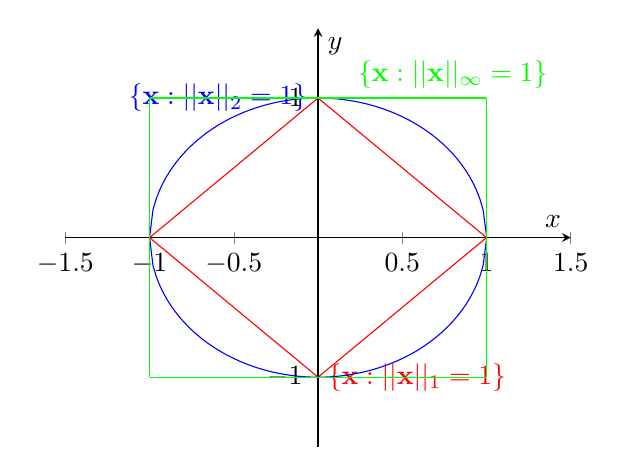
\begin{tikzpicture}
\begin{axis}[xmin=-1.5, xmax=1.5, ymin=-1.5, ymax=1.5, 
axis lines= middle, 
xlabel= $x$, 
ylabel= $y$,]
\addplot[color = red, samples = 100, domain = 0: 1]{-x+1};
\addplot[color = red, samples = 100, domain = -1: 0]{x+1};
\addplot[color = red, samples = 100, domain = -1: 0]{-x-1};
\addplot[color = red, samples = 100, domain = 0: 1]{x-1} node[right, pos = 0]{$\{ \vx : ||\vx||_1 = 1\}$};
\addplot[color = blue, samples = 100, domain = -1: 1]{sqrt(1-x^2)} node[left, pos = 0.5]{$\{ \vx : ||\vx||_2 = 1\}$};
\addplot[color = blue, samples = 100, domain = -1: 1]{-sqrt(1-x^2)};
\addplot[color = green, samples = 100, domain = -1: 1]{1} node[above, pos = 0.9]{$\{ \vx : ||\vx||_\infty = 1\}$};
\addplot[color = green, samples = 100, domain = -1: 1]{-1};
\addplot[samples=50, smooth, green] coordinates {(1, -1)(1, 1)};
\addplot[samples=50, smooth, green] coordinates {(-1, -1)(-1, 1)};
\end{axis}
\end{tikzpicture}
\end{tabular}
\end{center}
Remark: $||\vx||_p \leq ||\vx||_q$ if $p \geq q$
\end{enumerate}

\subsection{Matrix Vector Norm}
$\R^{m \times n}$ is a vector space. When we are talking about \textbf{matrix vector norm}, we are viewing $\R^{m \times n}$ as $\R^{mn}$ by vectorization. \begin{align*}
\begin{bmatrix}
x_{11} & x_{12}& \dots& x_{1n}\\
x_{21} & x_{22}& \dots& x_{2n}\\
\vdots & \vdots& \\
x_{m1} & x_{m2}& \dots& x_{mn}\\
\end{bmatrix} \rightarrow \begin{bmatrix}
x_{11}\\
\vdots\\
x_{m1}\\
x_{12}\\
\vdots\\
x_{m2}\\
\vdots\\
x_{1n}\\
\vdots\\
x_{mn}\\
\end{bmatrix}
\end{align*}
Then, we can define vector $p-$norm for $\R^{m \times n}$ as $$||A||_{p, vec} = (\sum_{i=1}^{m} \sum_{j=1}^{n} |a_{ij}|^p )^{\frac{1}{p}}$$
For example:
\begin{enumerate}
\item for $p=1$, $$||A||_{1, vec} = (\sum_{i=1}^{m} \sum_{j=1}^{n} |a_{ij}| )$$
\item for $p=\infty$, $$||A||_{\infty, vec} = \max_{i, j} |a_{ij}|$$
\end{enumerate}

\subsection{Matrix Norm}
When we are talking about \textbf{matrix norm}, we are viewing $\R^{m \times n}$ as linear transformation $\R^n \mapsto \R^m$. Then, we define matrix $p-$norm as $$||A||_{p} = \max_{\vx \neq 0, \vx \in \R^n} \dfrac{||A \vx||_p}{||\vx||_p}$$
For example:
\begin{enumerate}

\item For $p=2$,\\
\begin{tabular}{cc}
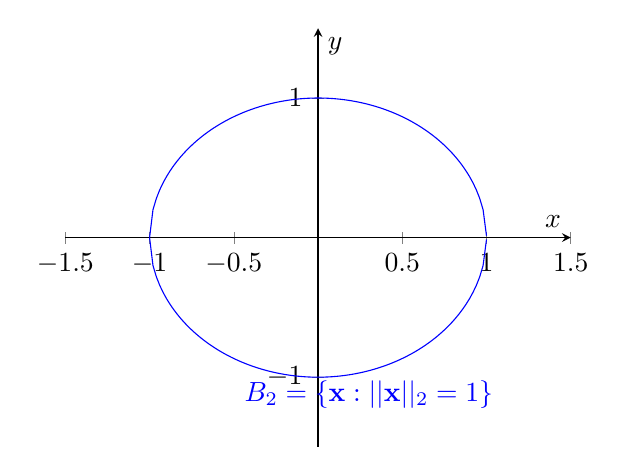
\begin{tikzpicture}
\begin{axis}[xmin=-1.5, xmax=1.5, ymin=-1.5, ymax=1.5, 
axis lines= middle, 
xlabel= $x$, 
ylabel= $y$,]
\addplot[color = blue, samples = 100, domain = -1: 1]{sqrt(1-x^2)};
\addplot[color = blue, samples = 100, domain = -1: 1]{-sqrt(1-x^2)}node[below, pos = 0.6]{$B_2 = \{ \vx : ||\vx||_2 = 1\}$};
\end{axis}
\end{tikzpicture}& 
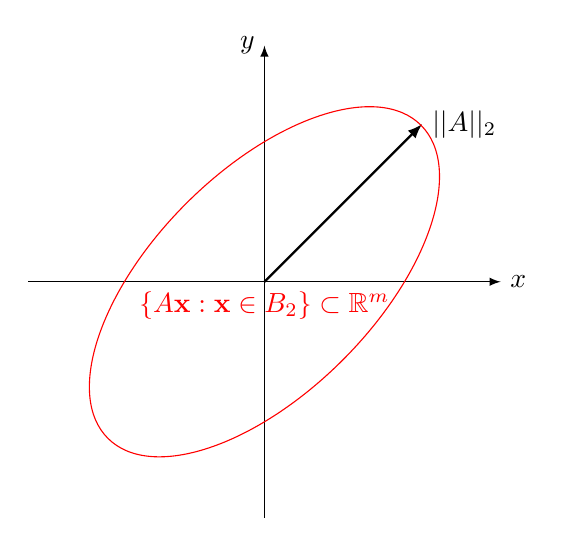
\begin{tikzpicture}[scale = 2]
\draw [-latex](-1.5, 0) -- (1.5, 0) node[right]{$x$};
\draw [-latex](0, -1.5) -- (0, 1.5) node[left]{$y$};
\draw [-latex, thick](0, 0) -- (1, 1) node[right]{$||A||_2$};
\draw[rotate=-45, color= red] (0,0) ellipse (20pt and 40pt) node[below]{$\{ A\vx : \vx \in B_2 \} \subset \R^m$};
\end{tikzpicture}
\end{tabular}

\item For $p=1$,\\
\begin{tabular}{cc}
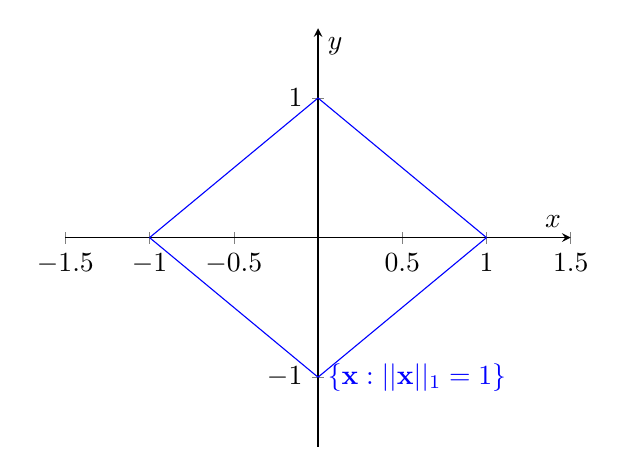
\begin{tikzpicture}
\begin{axis}[xmin=-1.5, xmax=1.5, ymin=-1.5, ymax=1.5, 
axis lines= middle, 
xlabel= $x$, 
ylabel= $y$,]
\addplot[color = blue, samples = 100, domain = 0: 1]{-x+1};
\addplot[color = blue, samples = 100, domain = -1: 0]{x+1};
\addplot[color = blue, samples = 100, domain = -1: 0]{-x-1};
\addplot[color = blue, samples = 100, domain = 0: 1]{x-1} node[right, pos = 0]{$ \{ \vx : ||\vx||_1 = 1\}$};
\end{axis}
\end{tikzpicture}& 
\begin{tikzpicture}[scale = 2]
\draw [-latex](-1.5, 0) -- (1.5, 0) node[right]{$x$};
\draw [-latex](0, -1.5) -- (0, 1.5) node[left]{$y$};
\draw [-latex, thick](0, 0)-- (1, 0) -- (1, 1) node[right]{$||A||_1$};
\draw [-, color= red] (-1, 1) -- (1, 1);
\draw [-, color= red] (1, 1) -- (0.8, -1);
\draw [-, color= red] (-1, 1) -- (-1.2, -1);
\draw [-, color= red] (-1.2, -1) -- (0.8, -1) node[below]{$\{ A \vx: \vx \in B_1\}$};
\end{tikzpicture}
\end{tabular}\\
Proposition: $\| A |\_{\infty} = \max_{ 1\leq i\leq m} \sum_{j=1}^{\infty} |a_{ij}|$\\
for example $$A = \begin{bmatrix}
2 & 1 & -1\\ 0&2 &4
\end{bmatrix} \in \R^{3 \times 2}$$ then $\|A\|_{\infty} = \max{|2|+|1|+|-1|, |0|+|2|+|4|} = 6$ 
\item For $p = \infty$, $$||A||_\infty = \max_{j \in \{1, 2, \cdots, m\}} \sum_{j=1}^{n} |a_{ij}|$$
\textit{proof:} it suffices to proof that $$\max_{\|A\|_{\infty} =1} \|A\|_{\infty} = \max_{ 1\leq i\leq m} \sum_{j=1}^{\infty} |a_{ij}|$$. We will proof that with two inequalities. 
\begin{enumerate}
\item $A = \begin{bmatrix}
a_1\\a_2\\ \vdots \\ a_m
\end{bmatrix}$ then $A\vx = \begin{bmatrix}
a_1 \vx \\ a_2 \vx \\ \vdots \\ a_{m} \vx
\end{bmatrix}$ \begin{align*}
\| A \|_{\infty} &= \max_{1\leq i\leq m} |a_i x|\\
&= \max_{1\leq i\leq m} |\sum_{j=1}^{n} a_{ij} x_j|\\
& \leq  \max_{1\leq i\leq m} \sum_{j=1}^{n}  |a_{ij}| |x_j|\\
&\leq  \max_{1\leq i\leq m} \sum_{j=1}^{n}  |a_{ij}|
\end{align*}
\item Choose a special $\vx$. Assume $\max_{1 \leq i \leq m} \sum_{j=1}^{n} |a_{ij}| = \sum_{j=1}^{n} |a_{i' j}|$ Let $\vx = \begin{bmatrix}
sign(a_{i'1}) \\  sign(a_{i'2}) \\ \vdots \\ sign(a_{i'n})
\end{bmatrix}$
\begin{align*}
\|A \vx\|_{\infty} &=  \max_{1 \leq i \leq m} |\sum_{j=1}^{n} a_{ij} x_j| \\
& \geq |\sum_{j=1}^{n} a_{i' j} x_j| \\
& = |\sum_{j=1}^{n} |a_{ij}|| \\
& = \sum_{j=1}^{n} |a_{ij}|\\
& = \max_{1 \leq i \leq m} \sum_{j=1}^{n} |a_{ij}|
\end{align*}
\end{enumerate}
By (a) and (b), we can conclude that $$\max_{\|A\|_{\infty} =1} \|A\|_{\infty} = \max_{ 1\leq i\leq m} \sum_{j=1}^{\infty} |a_{ij}|$$.
\item (Operator norm) For $p = 2$, \begin{align*}
||A||_2 &= \max_{||x||_2 = 1} ||A \vx||_2\\
&= \max_{||x||_2 = 1} ((A \vx)^T A \vx)^{\frac{1}{2}}\\
&= \max_{||x||_2 = 1} ( \vx^T A^T A \vx)^{\frac{1}{2}}\\
&= \text{Maximum Eigenvalues of } A^T A
\end{align*}
\end{enumerate}

We may also use different norms in $\R^n$ ($p-$norm) and $\R^m$ ($q-$norm). $$||A||_{p \to q} = \max_{\vx \neq \vzero, \vx = \R^n} \dfrac{||A \vx||_q}{||\vx||_p} = \max_{||\vx||_p = 1} ||A \vx||_q$$

\subsection{Other norms}
\begin{enumerate}
\item Nuclear norm\\
we can use different norms in $\mathbb{R}^n$ and $\R^m$. $$||A||_{p \to q} = \max_{||\vx||_p = 1} ||A\vx||_q$$
\item Norms on $C[a,b] = \{f: f \text{ is a continous function on } [a, b] \}$\\
For all $f \in C[a, b]$, we define 
\begin{enumerate}
\item $||f||_{\infty} = \max_{t \in [a,b]} |f(t)|$
\item $||f||_p = (\int_{a}^{b} |f(t)|^p dt)^{\frac{1}{p}}$ for $p \in \{1, 2, \cdots \}$
\end{enumerate}

\item Norms on $l_{\infty} = \{\mathbf{a}: \mathbf{a} \text{ is an infinite sequence and } \exists c > 0 \st |a_i| \leq c \,\, \forall i\}$
\begin{enumerate}
\item $||\mathbf{a}||_{\infty} = \sup_{i} |a_i|$
\item $||\mathbf{a}||_{p} = (\sum_{i=1}^{\infty} |a_i|^p) ^{\frac{1}{p}}$ but $||a||_{p}$ is indeed not a norm on $l_{\infty}$. We will proof that by a counter-example.
\begin{align*}
\mathbf{a} = \begin{bmatrix}
1\\ 1/2\\ 1/3\\ \vdots\\ 1/i\\ \vdots
\end{bmatrix} \in l_{\infty} \implies ||\mathbf{a}||_1 = \sum_{i=1}^{\infty} |a_i| = \sum_{i=1}^{\infty} {\frac{1}{i}} = + \infty
\end{align*}
If we just consider $l_{p} = \{\mathbf{a}: ||\mathbf{a}||_{p} =  (\sum_{i=1}^{\infty} |a_i|^p) ^{\frac{1}{p}}\}$, then we can just say $||\mathbf{a}||_p$ is a norm on $l_p$.

\textit{Remark:} Suppose $1 \leq p < q < \infty$, then $l_{p} \subset l_{q}$
\end{enumerate}
\end{enumerate}

\section{Case Study: K-means clustering, K-medians clustering}
\subsection{Clustering}
Suppose we are given $N$ vectors in $\R^n$, $$x_1, x_2, \cdots, x_N \in \R^n$$ we are going to divide them into $K$ different groups.\\
\textit{Remark: $\R^n$ here is used for simplicity, it can be replaced by any vector space.}\\
Applications: image clustering, text data clustering, recommendation system, etc.
\subsection{K-means clustering}
Recall that \texttt{Machine Learning = Representation + Evaluation + Optimization}, in the clustering case:
\begin{enumerate}
\item Representation:
\begin{enumerate}
\item $c_{i} - \text{the group that }\vx_i \text{ belongs to, for }i = 1, 2, \cdots, N$
\item $G_j  - \text{the indices of $\vx$'s that belongs to Group $j$}$ $$G_j = \{i | c_i = j \}, j = 1,2,\cdot, K$$
$$c_i, i = 1, \cdots, N \iff G_j, j=1, \cdots, K$$
\item $\vz_j - \text{the representation vector in }G_j , j = 1, \cdots K$\\
\textit{Remark: $\vz_j$ is not necessarily in $\{\vx_1, \cdots, \vx_N\}$}
\end{enumerate}
For example: we have $\vx_1 = (1,2)^T, \vx_2 = (3,4)^T, \vx_3 = (4,5)^T$, $K=2$ and $\vx_1, \vx_2 \in \text{Group 1}, \vx_3 \in \text{Group 2}$. Then with the above notations: $$c_1 = 1, c_2 =1, c_3 =2$$ $$G_1 = \{1,2\}, G_2 = \{3\}$$
\item Evaluation:
\begin{enumerate}
\item Within Group $j$: we want all the vectors within the group should be close to its representation vector $\vz_j$, that is to minimize $$J_j = \sum_{i \in G_j} ||\vx_i - \vz_j||_2 ^2$$
\item All groups: we want all of $J_i$'s to be small, that is to minimize $$J = J_1 + J_2 + \cdots + J_K$$
\end{enumerate}
Then, we want to solve the problem: $$\min_{G_1, \cdots, G_K; \vz_1, \cdots, \vz_K} J = \min_{G_1, \ldots, G_K; \vz_1, \ldots, \vz_K} \sum_{j=1}^{K} \sum_{i \in G_j} \|\vx_i - \vz_j\|_2^2$$
This is to find $G_1, \cdots, G_K$ and $\vz_1, \cdots \vz_2$ that minimizes $J$.
\item Optimization:\\
In this problem, we have to find two sets of unknowns $G_1, \cdots, G_K$ and $\vz_1, \cdots \vz_2$. We can use alternating minimization  to solve this problem.\\\\
Algorithm (Alternating minimization):\\
\begin{tabular}{lp{15cm}}
step 0:& Initialize $\vz_1, \cdots, \vz_k$\\
step 1:& Fix $\vz_1, \cdots, \vz_k$, solve the minimization with respect to $G_1, \cdots, G_K$. That is to solve $$\min_{G_1, \ldots, G_K} \sum_{j=1}^{K} \sum_{i \in G_j} \|\vx_i - \vz_j\|_2^2 -----(1)$$\\
step 2:& Fix $G_1, \cdots, G_K$, solve the minimization with respect to $\vz_1, \cdots, \vz_k$. That is to solve $$\min_{\vz_1, \cdots, \vz_k} \sum_{j=1}^{K} \sum_{i \in G_j} \|\vx_i - \vz_j\|_2^2 ------(2)$$\\
&(Repeat until stopping criterion meet)
\end{tabular}\\\\
How do we solve $(1)$, $(2)$?
\begin{enumerate}
\item[(1)] $$\sum_{j=1}^{K} \sum_{i \in G_j} \| \vx_i -\vz_j\|_2^2 = \sum_{j=1}^{K} \sum_{i \in G_j}\| \vx_i -\vz_{c_i}\|_2^2 = \sum_{i=1}^{N} \| \vx_i - \vz_{c_i}\|_2^2$$
Therefore, \begin{align*}
\min_{G_1, \ldots, G_K} \sum_{j=1}^{K} \sum_{i \in G_j} \|\vx_i - \vz_j\|_2^2 &\iff \min_{c_1, \cdots, c_N} \sum_{i=1}^{N} \|\vx_i - \vz_{c_i}\|_2^2\\
&\iff \min_{c_1, \cdots, c_N}  \|\vx_1 - \vz_{c_1} \|_2^2 + \cdots +\|\vx_N - \vz_{c_N} \|_2^2 \\
&\iff \min_{c_i \in \{1,2, \cdots, K\}} \|\vx_i - \vz_{c_i} \|_2^2 \text{ for } i = 1, 2, \cdots, N\\
&\iff c_i = \mathop{\arg\min}_{j \in {1, 2, \cdots, K}} \|\vx_i - \vz_j \|_2^2
\end{align*}
$\vx_i$ is assigned to the group whose representative is the closest to $\vx_i$. After that, we assign $$G_j = \{i | c_i = j\} \text{ for } j = 1, \cdots, K$$
\item[(2)] $$\sum_{j=1}^{K} \sum_{i \in G_j} \| \vx_i -\vz_j\|_2^2 = \sum_{i \in G_1} \|\vx_i - \vz_1 \|_2^2 + \cdots \sum_{i \in G_K} \|\vx_i - \vz_K \|_2^2$$
where each term only depends on $\vz_i$ and independent of $\vz_1, \cdots,\vz_{i-1},\vz_{i+1},\cdots,\vz_K$. Therefore, 
\begin{align*}
\sum_{j=1}^{K} \sum_{i \in G_j} \| \vx_i -\vz_j\|_2^2 &\iff \min_{\vz_j} \sum_{i \in G_j} \|\vx_i - \vz_j\|_2^2 \text{ for }j=1, \cdots, K\\
&\iff \vz_j = \mathop{\arg \min}_{\vz_j} \sum_{i \in G_j} \|\vx_i - \vz_j\|_2^2 \text{ for }j=1, \cdots, K
\end{align*}
Consider the case in $\R^n$, let $f(\vz) = \sum_{i \in G_j} \|\vx_i - \vz\|_2^2$
\begin{align*}
f(\vz) &= \sum_{i \in G_j} \|\vx_i - \vz\|_2^2\\
&= \sum_{i \in G_j} (\vx_i - \vz)^T (\vx_i - \vz)\\
&= \sum_{i \in G_j} \vx_i^T \vx_i -2\vx_i^T\vz + \vz^T \vz\\
&= |G_j|\vz^T \vz +\sum_{i \in G_j}\vx_i^T \vx_i -2\sum_{i \in G_j}\vx_i^T\vz
\end{align*} Then, $\nabla f(\vz)= 2|G_j|\vz -2\sum_{i \in G_j}\vx_i$. $\nabla^2 f(\vz) = 2 |G_j| I$. It is obvious that $\nabla^2 f(\vz)$ is positive definite. So, $f(\vz)$ is a convex function. By setting $\nabla f(\vz) = 0$, we can find the minimizer $\vz_{minimizer} = \frac{1}{|G_j|}\sum_{i \in G_j}\vx_i$ As a result, we can update $z_j = \frac{1}{|G_j|} \sum_{i \in G_j} \vx_i$, which is just the mean of $\vx_i$'s.
\end{enumerate}
\end{enumerate}

\subsection{K-medians Clustering}
In K-means Clustering, we used $2-$norm, what if we choose to use $1-$norm instead? $$\min_{G_1, \ldots, G_K; \vz_1, \ldots, \vz_K} \sum_{j=1}^{K} \sum_{i \in G_j} \|\vx_i - \vz_j\|_1$$ This will become the \textit{K-medians Clustering Algorithm}.

K-medians Clustering Algorithms:\\
\begin{tabular}{lp{15cm}}
step 0:& Initialize $\vz_1, \cdots, \vz_k$\\
step 1:& Fix $\vz_1, \cdots, \vz_k$, solve the minimization with respect to $G_1, \cdots, G_K$. That is to solve 
$$\min_{G_1, \ldots, G_K} \sum_{j=1}^{K} \sum_{i \in G_j} \|\vx_i - \vz_j\|_1 \iff c_i = \mathop{\arg \min}_{j \in \{1, \cdots K\}}\| \vx_i - \vz_j \|_1 \text{ For } i =1, \cdots, N$$\\
step 2:& Fix $G_1, \cdots, G_K$, solve the minimization with respect to $\vz_1, \cdots, \vz_k$. That is to solve $$\min_{\vz_1, \cdots, \vz_k} \sum_{j=1}^{K} \sum_{i \in G_j} \|\vx_i - \vz_j\|_1 \iff \min_{j} \sum_{i \in G_j} \| \vx_i - \vz_j\|_1 \text{ For } j= 1, \cdots, K$$ $$\vz_j = \text{entrywise-median}\{\vx_i | i \in G_j \} \text{ For } j = 1, \cdots, K$$\\
&(Repeat until stopping criterion meet)
\end{tabular}

\subsection{Comparison of K-means and K-medians}
Both mean and median can be using in clustering problem but median seems to have a better representation. 
\begin{enumerate}
\item Mean is sensitive to outliers.
\item Median is more robust to outliers.
\item In machine learning algorithms, $1-$norm distance is more robust than $2-$norm.
\end{enumerate}

\section{Limit and Convergence on vector space}
In calculus, we know that $\lim_{n \to \infty} a_n =  a \iff \lim_{n \to \infty} |a_n - a| = 0$. Is it also true on a vector space with a norm $\|\cdot\|$? The answer is yes.
\subsection{Limit and convergence on a normed vector space}

\end{document}